\documentclass{llncs}
%%%%%%%%%%%%%%%%%%%%%%%%%%%%%%%%%%%%%%%%%%%%%%%%%%%%%%%%%%%
%% package sillabazione italiana e uso lettere accentate
\usepackage[utf8]{inputenc}
\usepackage[english]{babel}
\usepackage[T1]{fontenc}
%%%%%%%%%%%%%%%%%%%%%%%%%%%%%%%%%%%%%%%%%%%%%%%%%%%%%%%%%%%%%

\usepackage{url}
\usepackage{xspace}

\makeatletter
%%%%%%%%%%%%%%%%%%%%%%%%%%%%%% User specified LaTeX commands.
\usepackage{manifest}

\makeatother


%%%%%%%
 \newif\ifpdf
 \ifx\pdfoutput\undefined
 \pdffalse % we are not running PDFLaTeX
 \else
 \pdfoutput=1 % we are running PDFLaTeX
 \pdftrue
 \fi
%%%%%%%
 \ifpdf
 \usepackage[pdftex]{graphicx}
 \else
 \usepackage{graphicx}
 \fi
%%%%%%%%%%%%%%%
 \ifpdf
 \DeclareGraphicsExtensions{.pdf, .jpg, .tif}
 \else
 \DeclareGraphicsExtensions{.eps, .jpg}
 \fi
%%%%%%%%%%%%%%%

\newcommand{\java}{\textsf{Java}}
\newcommand{\contact}{\emph{Contact}}
\newcommand{\corecl}{\texttt{corecl}}
\newcommand{\medcl}{\texttt{medcl}}
\newcommand{\msgcl}{\texttt{msgcl}}
\newcommand{\android}{\texttt{Android}}
\newcommand{\dsl}{\texttt{DSL}}
\newcommand{\jazz}{\texttt{Jazz}}
\newcommand{\rtc}{\texttt{RTC}}
\newcommand{\ide}{\texttt{Contact-ide}}
\newcommand{\xtext}{\texttt{XText}}
\newcommand{\xpand}{\texttt{Xpand}}
\newcommand{\xtend}{\texttt{Xtend}}
\newcommand{\pojo}{\texttt{POJO}}
\newcommand{\junit}{\texttt{JUnit}}

\newcommand{\action}[1]{\texttt{#1}\xspace}
\newcommand{\code}[1]{{\small{\texttt{#1}}}\xspace}
\newcommand{\codescript}[1]{{\scriptsize{\texttt{#1}}}\xspace}

% Cross-referencing
\newcommand{\labelsec}[1]{\label{sec:#1}}
\newcommand{\xs}[1]{\sectionname~\ref{sec:#1}}
\newcommand{\xsp}[1]{\sectionname~\ref{sec:#1} \onpagename~\pageref{sec:#1}}
\newcommand{\labelssec}[1]{\label{ssec:#1}}
\newcommand{\xss}[1]{\subsectionname~\ref{ssec:#1}}
\newcommand{\xssp}[1]{\subsectionname~\ref{ssec:#1} \onpagename~\pageref{ssec:#1}}
\newcommand{\labelsssec}[1]{\label{sssec:#1}}
\newcommand{\xsss}[1]{\subsectionname~\ref{sssec:#1}}
\newcommand{\xsssp}[1]{\subsectionname~\ref{sssec:#1} \onpagename~\pageref{sssec:#1}}
\newcommand{\labelfig}[1]{\label{fig:#1}}
\newcommand{\xf}[1]{\figurename~\ref{fig:#1}}
\newcommand{\xfp}[1]{\figurename~\ref{fig:#1} \onpagename~\pageref{fig:#1}}
\newcommand{\labeltab}[1]{\label{tab:#1}}
\newcommand{\xt}[1]{\tablename~\ref{tab:#1}}
\newcommand{\xtp}[1]{\tablename~\ref{tab:#1} \onpagename~\pageref{tab:#1}}
% Category Names
\newcommand{\sectionname}{Section}
\newcommand{\subsectionname}{Subsection}
\newcommand{\sectionsname}{Sections}
\newcommand{\subsectionsname}{Subsections}
\newcommand{\secname}{\sectionname}
\newcommand{\ssecname}{\subsectionname}
\newcommand{\secsname}{\sectionsname}
\newcommand{\ssecsname}{\subsectionsname}
\newcommand{\onpagename}{on page}

\newcommand{\xauthA}{Alessandro Bagnoli }
\newcommand{\xauthB}{Filippo Nicolini }
\newcommand{\xauthC}{Luca Pascucci }
\newcommand{\xfaculty}{II Faculty of Engineering}
\newcommand{\xunibo}{Alma Mater Studiorum -- University of Bologna}
\newcommand{\xaddrBO}{viale Risorgimento 2}
\newcommand{\xaddrCE}{via Sacchi 3}
\newcommand{\xcityBO}{40136 Bologna, Italy}
\newcommand{\xcityCE}{47023 Cesena, Italy}

%
% Comments
%
%%% \newcommand{\todo}[1]{\bf{TODO:}\emph{#1}}


\begin{document}

\title{Final Task 2016 \\ Software Engineering
 process report}

\author{\xauthA, \xauthB \and \xauthC}
%%\author{\xauthA}

\institute{%
  \xunibo\\\xaddrCE, \xcityCE\\\email{\{alessandro.bagnoli4, filippo.nicolini2, luca.pascucci\}@studio.unibo.it}
%%%  \xunibo\\\xaddrCE, \xcityCE\\\email\ nameA.studentA@studio.unibo.it
}

\maketitle

%% \begin{abstract}
%% \footnotesize
%%This a Latex template to be used for the reports of Software Engineering.
%%\keywords{Software engineering, managed software development, reports, ....}
%%\end{abstract}

%%% \sloppy

\section{Introduction}
\labelsec{intro}
This report describes the process to develop a system composed by a robot, one or multiple sonar and a radar. It includes all the different steps needed to analyse, prototype and implement the system, with a better definition of itself in the "Goals" and "Requirements" sections and show the main issues that occur in a heterogeneous and distributed environment.
\section{Vision}
\labelsec{Vision}
Below a list of values learned in this course:
\begin{itemize}
	\item A design without specifications cannot be right or wrong, it can only be surprising!
	\item There is non code without a project, no project without problem analysis and no problem without requirements.
	\item The question is how to make them explicit, effective and reusable.
	\item A feature does not exist unless a test validates that it functions.
	\item Analyse a little. Design a little. Code a little. Test what you can.
\end{itemize}
Our vision ....

\section{Goals}
\labelsec{Goals}
\section{Requirements}
\labelsec{Requirements}
\section{Requirement analysis}
\labelsec{ReqAnalysis}

\subsection{User stories}
\labelssec{UserStories}
%\textbf{As a} user, \textbf{I want} to place the robot at the beginning point, and make it start running. \\
%\textbf{As a} user, \textbf{I can} stop the robot at any time, and make it restart placing it at the beginning point. \\
%\textbf{As a} user, \textbf{I want} to see the photos taken by the robot during its walking. \\
%\textbf{As a} user, \textbf{I want} to see the sonars data on a graphical user interface.
%\\\\
\textbf{As a} user, \textbf{I want} (R1) to place the robot at the beginning point, and make it start running to a prefixed area. While the robot is moving and reaches the area in front of a sonar, \textbf{I want} that (R2) the robot stops turn left about 90$^\circ$, start blinking a led, take the photo of the world in front of it, send the photo to the console, turn right about 90$^\circ$ to compensate the previous rotation, stop blinking the led and continues its movement to the prefixed area. While the robot is moving \textbf{I want} (R3) to be able to stop it, and make it restart placing it at the beginning point. \textbf{As a} user \textbf{I want} (R4) to see the sonar data on a graphical user interface associated to a console running on a conventional PC. \textbf{As a} user \textbf{I want} that (R5) the system evaluate the expression and play an alarm sound when its value is less than a prefixed value, stopping the robot. \textbf{As a} user \textbf{I want} that (R6) the robot can stop itself when an obstacle is detected by the sonar in front of it.
\subsection{Scenarios}
\labelssec{Scenarios}
\subsection{(Domain)model}
A domain model is a conceptual model that incorporate behaviour and data. It can be used to solve problems related to that domain.
\subsection{Test plan}
The test plan include integration test that is used to check that the integration between the components takes place in the right way.
\section{Problem analysis}
\labelsec{ProblemAnalysis}
Our technological hypothesis is JAVA and Object Oriented Programming. We
will show that we need to develop a new infrastructure because the only features
offered by the programming language chosen are not enough. To keep our code
well developed, scalable, efficient and maintainable, we will use the most known
development patterns. We must define an interaction language, that needs a
communication standard.
\subsection{Logic architecture}
The logic architecture of a (distributed) software system can be specified by a custom (domain specific) language. In this case scenario, \textit{qa} DSL has turned to be very helpful. The main aim of the custom language qa is to give more expressive power than UML for the definition of system models, both during the problem analysis phase and during the project phase. The language qa allows us to specify:
\begin{itemize}
	\item the main components (\textbf{QActor}) of a system software system
	\item how the components are mapped into computational nodes (\textbf{Context})
	\item how the components exchange information (using \textbf{Messages} and \textbf{Events})
	\item how each component works (\textbf{behaviour})
\end{itemize}
Here is the logic architecture of the system described using qa language:
\lstinputlisting{list/robotSystem.ddr}
\subsection{Abstraction gap}
During the problem analysis we considered Java as our technological hypothesis.
We realized that Java’s unique communication tool is procedure calls, with
OO paradigm it becomes really difficult to implement modular communication
where entities are completely independent and loosely coupled. We need a new
way to let our components interact. In agreement with our vision, we understand
that the best way to overcome this problem is to develop a new software
infrastructure that will map more strictly to our model representation than Java
paradigms. This infrastructure will be used not only in this project, but every
future developed process that will have the same needs because, according to
our visions, we want to develop reusable code.
Our platform must offer some functionalities. First of all we need a formal definition
of a System:
a System is one or more active entities that interact to reach some goal or provide
some functionalities. A system is composed by one or more Contexts, a Contexts
identifies a logical location at deployment time. The System enables the communication
between the entities and synchronizes them so Entities must interact
using the System only. In this way a System can be concentrated or distributed
seamlessly for the application designer. Defined this general perspective we can
introduce two paradigms:
\begin{itemize}
	\item Message Based Programming
	\item Event Based Programming
\end{itemize}
\textbf{Message Based Programming:} to introduce message based programming we
need to define the entities that can exchange messages. We will call these entities
QActors.
QActors in our platform are not message-driven but message-based. The core
difference between message driven and message based is that message driven
systems can be only reactive to messages instead of being able to decide when
messages and which messages are functional to evaluate. In this way we can
model not only reactive entities but also proactive ones. QActors live in a context
and they can communicate with other QActors using different communication
primitives, like \textit{dispatch}: an asynchronous message without returning information. \\
QActors can receive messages using the receive message primitives, like \textit{receiveMessage} which extracts the first message from the actor message queue. \\\\
\textbf{Event Based Programming}: we needed to define the concept of events as pervasive messages that are spread in the system. The message passing paradigm
lacks of this feature because all messages are point to point. Events are a form
of asynchronous communication that is not point to point. In our system our
entities can declare to be interested in an event, when that event will be emitted
the entities can react in some way.
When we introduced proactive QActors we realized that we needed the concept
of Plan. A Plan is a sequence of actions (you can see actions as programming
language instructions), every plan has its own logic and can switch to a different
plan. When the execution of a plan reaches its end it can specify if the
previous plan must continue its execution or suspend it. This abstraction was
lacking of the better part of message/event driven programming: reactivity. This
gap is filled by Asynchronous Actions. Asynchronous Actions are tipically time
consuming actions that can be executed in blocking or non-blocking way. When
executing an asynchronous action its execution can be interrupted by specified
events and the QActor must react executing the associated plan. The logic of
plan switching is defined as above. QActors are able to execute actions in two
ways:
\begin{itemize}
	\item executing compiled code
	\item interpreting meta code on the fly
\end{itemize} 
Adding the possibility to interpret code on the fly permits to the QActor to enrich
its behaviour during runtime. The just described platform will be realized with
Java Programming Language (our technologic assumption) but will be made
to be interoperable with other technologies by the extensive use of text-based
messages using the standard socket technology.
On top of the API offered by the platform we’ll realize a DSL using the xtext
framework. With the use of such tool we’ll generate a declarative language that
will provide two main benefits:
\begin{itemize}
	\item a formal and human readable language to describe the problem analysis,
	entities interactions and system topology;
	\item code generation to be able to customize and execute the artifacts generated by the DSL interpretation.
\end{itemize}
With such tools in mind we can reimagine the traditional problem analysis
techniques and tackle the problems in a formal and more convenient way.
\subsection{Risk analysis}
\section{Work plan}
\labelsec{wplan}
\section{Project}
\labelsec{Project}
The purpose of the project phase is to refine the logical architecture of the system, considering all the binding aspects that have been ignored in the previous phases.
\subsection{Structure}
\subsection{Interaction}
A QActor can interact with others (local or remote) QActor by sending/receiving messages. A QActor can also emit or sense events.
\begin{figure}[h]
	\centering
	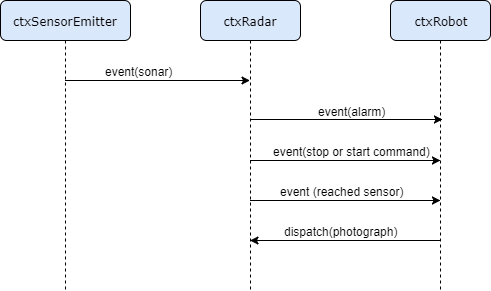
\includegraphics[width=\linewidth]{interaction.png}
	\caption{Interactions between the three contexts.}
\end{figure}
\subsection{Behaviour}
A QActor is an active (autonomous) entity that runs in parallel with the other actors defined in the same or in other contexts. The behaviour of a QActor can be expressed as a Moore Finite State Machine (M-FSM). Each state of the M-FSM can be expressed by a \textbf{Plan} which is composed of a sequence of \textbf{actions}.
Here are the finite state machines of our system:
\begin{figure}[h]
	\centering
	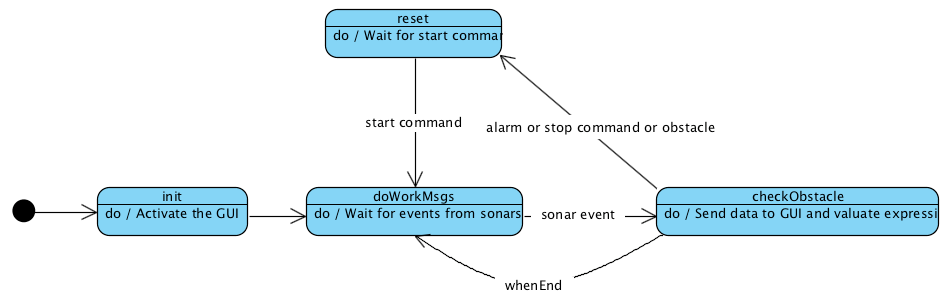
\includegraphics[width=\linewidth]{radargui.png}
	\caption{FSM for the radargui actor.}
\end{figure}
\begin{figure}[h]
	\centering
	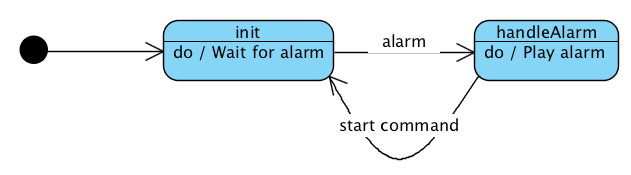
\includegraphics[width=9cm]{alarmhandler.png}
	\caption{FSM for the alarmhandler actor.}
\end{figure}
\begin{figure}[h]
	\centering
	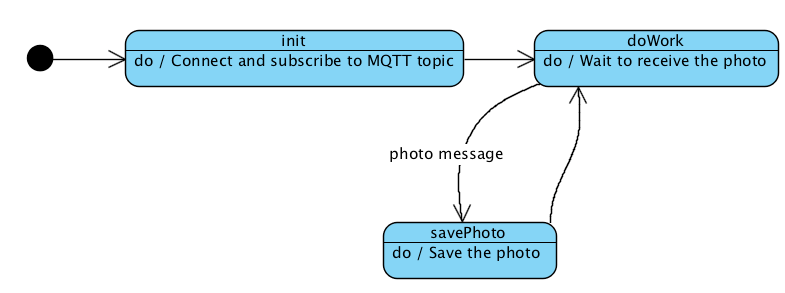
\includegraphics[width=9cm]{photoreceiver.png}
	\caption{FSM for the photoreceiver actor.}
\end{figure}
\begin{figure}[h]
	\centering
	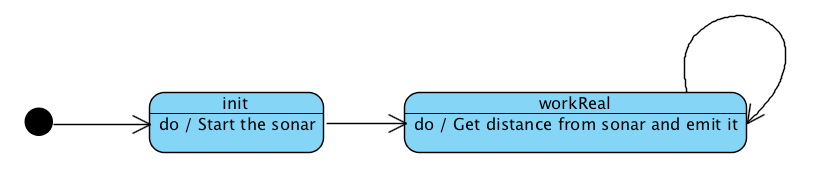
\includegraphics[width=9cm]{sensorsonar.png}
	\caption{FSM for the sensorsonar actor.}
\end{figure}
\begin{figure}[h]
	\centering
	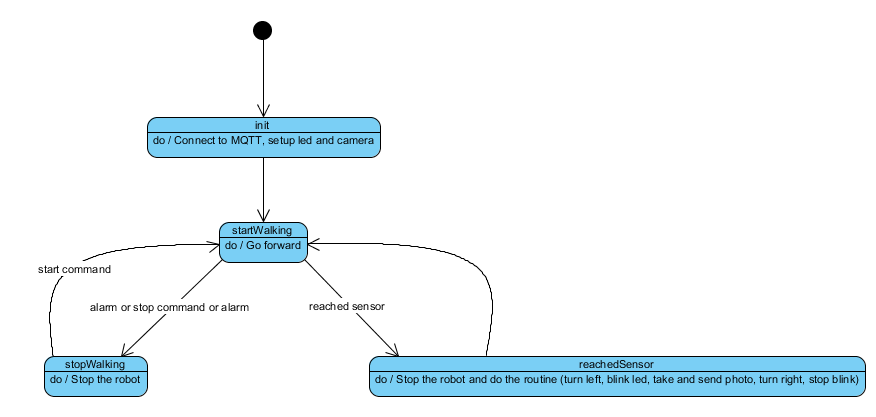
\includegraphics[width=\linewidth]{robotactor.png}
	\caption{FSM for the robot actor.}
\end{figure}
\clearpage
\section{Implementation}
\labelsec{Implementation}
\subsection{Radar}
The console part of the radar is implemented as a web page, which is automatically generated in the \lstinline[columns=fixed]{srcMore} directory in a package associated with each Context when the \textbf{-httpserver} flag for a Context is set. It is implemented by a HTTP web-socket server working on port 8080. This interface emits different kind of events. For example, the Start button emits the event  \lstinline[columns=fixed]{cmd : cmd(start)}.
\begin{figure}[h]
	\centering
	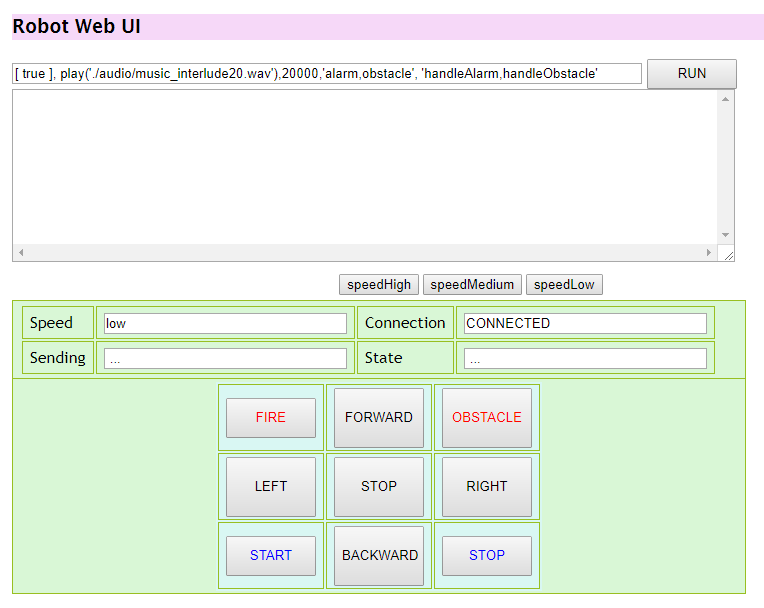
\includegraphics[width=\linewidth]{webconsole.png}
	\caption{Web console.}
\end{figure}
\\
The GUI part of the radar (where the sonars data are shown) is implemented using specific libraries provided by the software house.
\subsection{Led blinking}
The blink of the led has to be asynchronous, so that while the led is blinking, the robot can continue its operations without being blocked. In order to do so, the led is implemented as a \lstinline[columns=fixed]{SituatedActiveObject} supplied by the software house.
\lstinputlisting[style=java]{list/BlinkAsynch.java}
\subsection{Transmission of images through MQTT}
For the photo shoot through the camera, we used an open source library found on Github, called \textbf{JRPiCam} which wraps the commands needed to take a photo. Once the photo is acquired, it is converted in a String encoded with \textbf{Base64} encoding and then published on the \textbf{MQTT} broker, with a specified topic. The radar running on PC will have to decode the String received through MQTT in order to rebuild the image and then save it locally.
\lstinputlisting[style=java]{list/Camera.java}
\lstinputlisting[style=java]{list/Photoreceiver.java}
All the sonars, either on the path or on the robot, retreive the distances executing a C program called \lstinline[columns=fixed]{SonarAlone}, provided by the sofware house.
\lstinputlisting[style=java]{list/Sensorsonar.java}
\section{Testing}
\labelsec{testing}
The system was initially tested using the \textit{robotMock} abstraction locally. The robot mock is totally equivalent to the ddr robot from the point of view of the behaviours, but uses simulated sensory data and generates prints instead of sending electric signals to the pins connected to the motors. The system has successfully passed the testing phase.
\section{Deployment}
\labelsec{Deployment}
\section{Maintenance}
\labelsec{Maintenance}
\newpage
See \cite{natMol09} until page 11 (\texttt{CMM}) and pages 96-105.

%===========================================================================
\section{Information about the authors}
\labelsec{Author}

\vskip.5cm
%%% \begin{figure}
\begin{tabular}{ | c |  }
	\hline
	% after \\: \hline or \cline{col1-col2} \cline{col3-col4} ...
	Photo of the author 
	\\
	\hline
	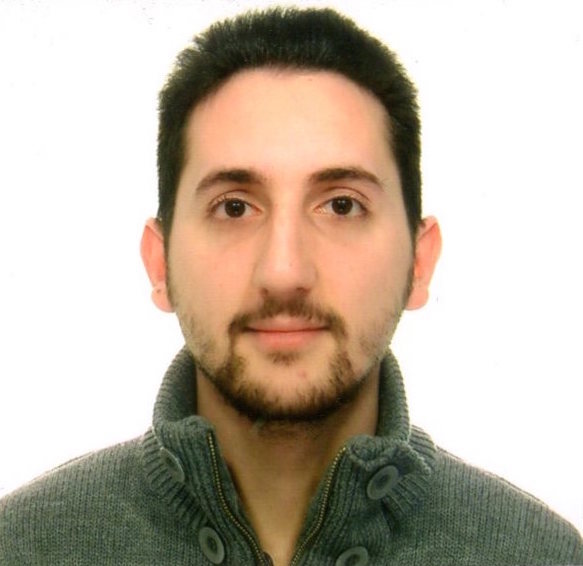
\includegraphics[scale = 0.7]{img/LucaPascucci.jpg}
	\\
	\hline
\end{tabular}


%===========================================================================


%%% \begin{itemize}
%%% \item Titolo di studio:\\ \\
%%% \item Interessi particolari:\\ \\
%%% \item Ha sostenuto fino ad oggi il seguente numero di esami:\\ \\
%%% \item Deve ancora sostenere i seguenti esami del I anno:\\ \\
%%% \item Prevede di svolgere un tirocinio presso:\\ \\
%%% \item Prevede di laurearsi nella sessione:\\ \\
%%% \item Intende proseguire gli studi per conseguire: \\  \\  \\
%%%   	presso la sede universitaria di: \\ \\
%%% \item Intende entrare subito nel mondo del lavoro presso : \\ \\
%%% \end{itemize}

 
\appendix


\bibliographystyle{abbrv}
\bibliography{biblio}

\end{document}












